\documentclass[letterpaper,11pt]{article}

\usepackage{latexsym}
\usepackage[empty]{fullpage}
\usepackage{titlesec}
\usepackage{marvosym}
\usepackage[usenames,dvipsnames]{color}
\usepackage{verbatim}
\usepackage{enumitem}
\usepackage[hidelinks]{hyperref}
\usepackage{csquotes}
\usepackage[english]{babel}
\usepackage{graphicx}
\usepackage{multirow}
\usepackage[style=geschichtsfrkl,sorting=none]{biblatex}
\addbibresource{pubs.bib}

\newcommand{\nameuse}[1]{%
\def\do##1{\settoggle{blx@use##1}{#1}}%
\dolistcsloop{blx@datamodel@names}}

% \pagestyle{fancy}
% \fancyhf{} % clear all header and footer fields
% \fancyfoot{}
% \renewcommand{\headrulewidth}{0pt}
% \renewcommand{\footrulewidth}{0pt}

% Adjust margins
\addtolength{\oddsidemargin}{-0.5in}
\addtolength{\evensidemargin}{-0.5in}
\addtolength{\textwidth}{1in}
\addtolength{\topmargin}{-.5in}
\addtolength{\textheight}{1.0in}

\urlstyle{same}

\raggedbottom
\raggedright
\setlength{\tabcolsep}{0in}

\newcommand{\rom}[1]{\uppercase\expandafter{\romannumeral #1\relax}}

% Sections formatting
\titleformat{\section}{
	\vspace{-4pt}\scshape\raggedright\large
}{}{0em}{}[\color{black}\titlerule \vspace{-5pt}]

%--------------------------------------
% Custom commands
\newcommand{\resumeItem}[2]{
	\item\small{
		\textbf{#1}{: #2 \vspace{-2pt}}
	}
}

\newcommand{\resumeSubheading}[5]{
	\vspace{-1pt}\item
	\begin{tabular*}{0.97\textwidth}[t]{ll@{\extracolsep{\fill}}r}
		\multirow{2}{*}{#1} & \textbf{#2} & #3 \\
		& \textit{\small#4} & \textit{\small #5} \\
	\end{tabular*}\vspace{-5pt}
}

\newcommand{\resumeSubItem}[2]{\resumeItem{#1}{#2}\vspace{-4pt}}

\renewcommand{\labelitemii}{$\circ$}

\newcommand{\resumeSubHeadingListStart}{\begin{itemize}[leftmargin=*,label=]}
		\newcommand{\resumeSubHeadingListEnd}{\end{itemize}}
\newcommand{\resumeItemListStart}{\begin{itemize}[label=$\bullet$]}
		\newcommand{\resumeItemListEnd}{\end{itemize}\vspace{-5pt}}

%--------------------------------------
%%%%%%%%%%  CV STARTS HERE  %%%%%%%%%%%


\begin{document}

%--------------HEADING-----------------
\begin{tabular*}{\textwidth}{l@{\extracolsep{\fill}}r}
	\textbf{\href{http://localhost}{\Large Daniel Nakhimovich}} & Email : \href{dnahimov@gmail.com}{dnahimov@gmail.com}\\
	\href{http://localhost}{-----------------------------------------} & Mobile : +1-551-795-5019 \\
\end{tabular*}


%-------------EDUCATION----------------
\section{Education}
\resumeSubHeadingListStart
\resumeSubheading
{
\includegraphics[width=23pt]{./images/rutgers.png}}
{Rutgers University}{New Brunswick, NJ}
{Doctor of Philosophy in Robotics; GPA: 3.90}{Sept 2019 -- May 2024}
\resumeSubheading
{
\includegraphics[width=23pt]{./images/cooper.png}}
{The Cooper Union}{New York, NY}
{Bachelor of Engineering in Electrical Engineering; GPA: 3.55}{Sept 2015 -- May. 2019}
\resumeSubHeadingListEnd


%--------------RESEARCH----------------

%-------------EXPERIENCE---------------
\section{Experience}
\resumeSubHeadingListStart
\resumeSubheading
{
\includegraphics[width=23pt]{./images/dimacs.png}}
{DIMACS}{Piscataway, NJ}
{Undergraduate Researcher}{Summer 2018 -- 2019}
\resumeItemListStart
\resumeItem{Support}
{This work was partially supported by the Computer-Human Graph TeleDiscovery grant (IIS-1563971) under the direction of James Abello.}
\resumeItem{k-connectivity}
{k-connectivity is a connectivity measure for graphs. Designed two algorithms for finding approximations of minimum seperating sets of a graph in order to perform efficient graph decomposition for data visualization.}
\resumeItem{Graph Peeling}
{Graph Peeling is the iterative process of removing vertices from a graph. Explored properties of various graph peeling techniques and designed a new peeling algorithm (wave decomposition) in order to decompose very large graphs efficiently.}
\resumeItemListEnd

\resumeSubheading
{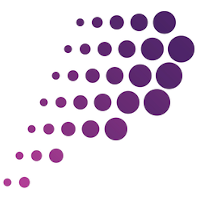
\includegraphics[width=23pt]{./images/pulsepoint.png}}
{PulsePoint}{New York, NY}
{TechOps Intern}{Summer 2017}
\resumeItemListStart
\resumeItem{QPS Monitoring}
{QPS stands for queries per second. Optimized application metric collection/alerting to reduce the false positve rate of QPS drops.}
\resumeItem{System Integrity}
{Automated the backup and data verification of large (\url{~}100GB) databases.}
\resumeItemListEnd

\resumeSubheading
{
\includegraphics[width=23pt]{./images/conceptheca.png}}
{Conceptheca}{Fair Lawn, NJ}
{Mobile Application Developer}{2015 -- 2016}
\resumeItemListStart
\resumeItem{Blood-loss}
{A mobile application on Android/iOS for doctors that calculates the maximum allowable blood-loss that a patient can undergo before reaching critical condition}
\resumeItem{JAM Fractals}
{A mobile game on Android OS that allows a player to mix ingredients to form seemingly random and chaotic fractal images}
\resumeItem{Sepsis Clock}
{An iOS application to help doctors keep track of the time and completion progress of the procedures to treat patients with septic shock}
\resumeItemListEnd
\resumeSubHeadingListEnd


%--------------PROJECTS----------------
\section{Projects}
\resumeSubHeadingListStart
\resumeSubItem{skEye Net}
{Wireless eye tracking / gaze estimation headset that works in realtime; $1^{st}$ place at HackCooper 2018}
\resumeSubItem{OpenSesame}
{Open source cryptographic co-processor implemented on an FPGA}
\resumeSubItem{pass2act}
{Passive to active sentence transformer built using spaCy's dependency tree parser}
\resumeSubItem{biboch}
{Bitboard checkers implementation with an AI that performs a fast alpha/beta search on the game tree}
\resumeSubItem{8-bit processor}
{Custom 8-bit instruction set architecture written in verilog}
\resumeSubHeadingListEnd

%--------------------------------------

%------------AFFILIATIONS--------------
% \section{Organizations}
%         \resumeSubHeadingListStart
%                 \resumeSubItem{Rutgers Astronomical Society}
%                 {}
%         \resumeSubHeadingListEnd

%--------------------------------------

%------------PUBLICATIONS--------------
\section{Publications}
% \resumeSubHeadingListStart
% \resumeSubItem{[Wafr58]}
% {Rahul Shome, Daniel Nakhimovich, and Kostas E. Bekris, ``Pushing the Boundaries of Asymptotic Optimality in Integrated Task and Motion Planning'' in \textit{Submitted to The 14th International Workshop on the Algorithmic Foundations of Robotics}, WAFR, (2020).}
% \resumeSubItem{[BigVis3]}
% {James Abello and Daniel Nakhimovich, ``Graph Waves'' in \textit{International Workshop on Big Data Visual Exploration and Analytics with EDBT/ICDT}, BigVis, (2020).}
% \resumeSubHeadingListEnd

\nocite{*}
\renewcommand*{\section}[2]{}
\renewcommand*{\intitlepunct}{\addspace}
\DeclareFieldFormat{title}{\mkbibbold{#1}}
\DeclareFieldFormat{journaltitle}{\mkbibemph{#1\isdot}}
\DeclareFieldFormat{issuetitle}{\mkbibemph{#1}}
\DeclareFieldFormat{maintitle}{\mkbibemph{#1}}
\DeclareFieldFormat{booktitle}{\mkbibemph{#1}}
\nameuse{false}
\printbibliography

%--------------------------------------
\end{document}
